% Options for packages loaded elsewhere
\PassOptionsToPackage{unicode}{hyperref}
\PassOptionsToPackage{hyphens}{url}
%
\documentclass[
]{article}
\usepackage{lmodern}
\usepackage{amssymb,amsmath}
\usepackage{ifxetex,ifluatex}
\ifnum 0\ifxetex 1\fi\ifluatex 1\fi=0 % if pdftex
  \usepackage[T1]{fontenc}
  \usepackage[utf8]{inputenc}
  \usepackage{textcomp} % provide euro and other symbols
\else % if luatex or xetex
  \usepackage{unicode-math}
  \defaultfontfeatures{Scale=MatchLowercase}
  \defaultfontfeatures[\rmfamily]{Ligatures=TeX,Scale=1}
\fi
% Use upquote if available, for straight quotes in verbatim environments
\IfFileExists{upquote.sty}{\usepackage{upquote}}{}
\IfFileExists{microtype.sty}{% use microtype if available
  \usepackage[]{microtype}
  \UseMicrotypeSet[protrusion]{basicmath} % disable protrusion for tt fonts
}{}
\makeatletter
\@ifundefined{KOMAClassName}{% if non-KOMA class
  \IfFileExists{parskip.sty}{%
    \usepackage{parskip}
  }{% else
    \setlength{\parindent}{0pt}
    \setlength{\parskip}{6pt plus 2pt minus 1pt}}
}{% if KOMA class
  \KOMAoptions{parskip=half}}
\makeatother
\usepackage{xcolor}
\IfFileExists{xurl.sty}{\usepackage{xurl}}{} % add URL line breaks if available
\IfFileExists{bookmark.sty}{\usepackage{bookmark}}{\usepackage{hyperref}}
\hypersetup{
  pdftitle={Who Gets Constituent Service?},
  pdfauthor={Rochelle Snyder, Eleanor Neff Powell, Devin Judge-Lord, Justin Grimmer},
  hidelinks,
  pdfcreator={LaTeX via pandoc}}
\urlstyle{same} % disable monospaced font for URLs
\usepackage[margin=1in]{geometry}
\usepackage{color}
\usepackage{fancyvrb}
\newcommand{\VerbBar}{|}
\newcommand{\VERB}{\Verb[commandchars=\\\{\}]}
\DefineVerbatimEnvironment{Highlighting}{Verbatim}{commandchars=\\\{\}}
% Add ',fontsize=\small' for more characters per line
\usepackage{framed}
\definecolor{shadecolor}{RGB}{248,248,248}
\newenvironment{Shaded}{\begin{snugshade}}{\end{snugshade}}
\newcommand{\AlertTok}[1]{\textcolor[rgb]{0.94,0.16,0.16}{#1}}
\newcommand{\AnnotationTok}[1]{\textcolor[rgb]{0.56,0.35,0.01}{\textbf{\textit{#1}}}}
\newcommand{\AttributeTok}[1]{\textcolor[rgb]{0.77,0.63,0.00}{#1}}
\newcommand{\BaseNTok}[1]{\textcolor[rgb]{0.00,0.00,0.81}{#1}}
\newcommand{\BuiltInTok}[1]{#1}
\newcommand{\CharTok}[1]{\textcolor[rgb]{0.31,0.60,0.02}{#1}}
\newcommand{\CommentTok}[1]{\textcolor[rgb]{0.56,0.35,0.01}{\textit{#1}}}
\newcommand{\CommentVarTok}[1]{\textcolor[rgb]{0.56,0.35,0.01}{\textbf{\textit{#1}}}}
\newcommand{\ConstantTok}[1]{\textcolor[rgb]{0.00,0.00,0.00}{#1}}
\newcommand{\ControlFlowTok}[1]{\textcolor[rgb]{0.13,0.29,0.53}{\textbf{#1}}}
\newcommand{\DataTypeTok}[1]{\textcolor[rgb]{0.13,0.29,0.53}{#1}}
\newcommand{\DecValTok}[1]{\textcolor[rgb]{0.00,0.00,0.81}{#1}}
\newcommand{\DocumentationTok}[1]{\textcolor[rgb]{0.56,0.35,0.01}{\textbf{\textit{#1}}}}
\newcommand{\ErrorTok}[1]{\textcolor[rgb]{0.64,0.00,0.00}{\textbf{#1}}}
\newcommand{\ExtensionTok}[1]{#1}
\newcommand{\FloatTok}[1]{\textcolor[rgb]{0.00,0.00,0.81}{#1}}
\newcommand{\FunctionTok}[1]{\textcolor[rgb]{0.00,0.00,0.00}{#1}}
\newcommand{\ImportTok}[1]{#1}
\newcommand{\InformationTok}[1]{\textcolor[rgb]{0.56,0.35,0.01}{\textbf{\textit{#1}}}}
\newcommand{\KeywordTok}[1]{\textcolor[rgb]{0.13,0.29,0.53}{\textbf{#1}}}
\newcommand{\NormalTok}[1]{#1}
\newcommand{\OperatorTok}[1]{\textcolor[rgb]{0.81,0.36,0.00}{\textbf{#1}}}
\newcommand{\OtherTok}[1]{\textcolor[rgb]{0.56,0.35,0.01}{#1}}
\newcommand{\PreprocessorTok}[1]{\textcolor[rgb]{0.56,0.35,0.01}{\textit{#1}}}
\newcommand{\RegionMarkerTok}[1]{#1}
\newcommand{\SpecialCharTok}[1]{\textcolor[rgb]{0.00,0.00,0.00}{#1}}
\newcommand{\SpecialStringTok}[1]{\textcolor[rgb]{0.31,0.60,0.02}{#1}}
\newcommand{\StringTok}[1]{\textcolor[rgb]{0.31,0.60,0.02}{#1}}
\newcommand{\VariableTok}[1]{\textcolor[rgb]{0.00,0.00,0.00}{#1}}
\newcommand{\VerbatimStringTok}[1]{\textcolor[rgb]{0.31,0.60,0.02}{#1}}
\newcommand{\WarningTok}[1]{\textcolor[rgb]{0.56,0.35,0.01}{\textbf{\textit{#1}}}}
\usepackage{graphicx}
\makeatletter
\def\maxwidth{\ifdim\Gin@nat@width>\linewidth\linewidth\else\Gin@nat@width\fi}
\def\maxheight{\ifdim\Gin@nat@height>\textheight\textheight\else\Gin@nat@height\fi}
\makeatother
% Scale images if necessary, so that they will not overflow the page
% margins by default, and it is still possible to overwrite the defaults
% using explicit options in \includegraphics[width, height, ...]{}
\setkeys{Gin}{width=\maxwidth,height=\maxheight,keepaspectratio}
% Set default figure placement to htbp
\makeatletter
\def\fps@figure{htbp}
\makeatother
\setlength{\emergencystretch}{3em} % prevent overfull lines
\providecommand{\tightlist}{%
  \setlength{\itemsep}{0pt}\setlength{\parskip}{0pt}}
\setcounter{secnumdepth}{-\maxdimen} % remove section numbering

\title{Who Gets Constituent Service?}
\author{Rochelle Snyder, Eleanor Neff Powell, Devin Judge-Lord, Justin
Grimmer}
\date{}

\begin{document}
\maketitle

{
\setcounter{tocdepth}{2}
\tableofcontents
}
\begin{quote}
These plots can be found in the
\href{https://www.dropbox.com/home/CorRep/figs}{CorRep/figs} folder on
dropbox and the
\href{https://github.com/judgelord/correspondence/tree/master/APSA2020/Figs}{APSA2020/figs}
folder on github.
\end{quote}

\begin{Shaded}
\begin{Highlighting}[]
\KeywordTok{source}\NormalTok{(here}\OperatorTok{::}\KeywordTok{here}\NormalTok{(}\StringTok{"setup.R"}\NormalTok{))}

\KeywordTok{library}\NormalTok{(ggplot2); }\KeywordTok{theme\_set}\NormalTok{(}\KeywordTok{theme\_bw}\NormalTok{())}
  \KeywordTok{options}\NormalTok{(}
    \DataTypeTok{ggplot2.continuous.color =} \StringTok{"viridis"}\NormalTok{,}
    \DataTypeTok{ggplot2.continuous.fill =} \StringTok{"viridis"}
\NormalTok{  )}
\NormalTok{  scale\_color\_discrete \textless{}{-}}\StringTok{ }\ControlFlowTok{function}\NormalTok{(...)}
    \KeywordTok{scale\_color\_viridis\_d}\NormalTok{(...)}
\NormalTok{  scale\_fill\_discrete \textless{}{-}}\StringTok{ }\ControlFlowTok{function}\NormalTok{(...)}
    \KeywordTok{scale\_fill\_viridis\_d}\NormalTok{(...)}
\end{Highlighting}
\end{Shaded}

\begin{Shaded}
\begin{Highlighting}[]
\KeywordTok{load}\NormalTok{(here}\OperatorTok{::}\KeywordTok{here}\NormalTok{(}\StringTok{"data/all\_contacts.Rdata"}\NormalTok{))}
\NormalTok{d \textless{}{-}}\StringTok{ }\NormalTok{all\_contacts}

\NormalTok{d }\OperatorTok{\%\textless{}\textgreater{}\%}\StringTok{ }
\StringTok{    }\KeywordTok{mutate}\NormalTok{(}\DataTypeTok{TYPE =} \KeywordTok{replace\_na}\NormalTok{(TYPE, }\StringTok{"NA"}\NormalTok{),}
           \DataTypeTok{constituent =} \KeywordTok{ifelse}\NormalTok{(TYPE }\OperatorTok{==}\StringTok{ }\DecValTok{1}\NormalTok{, }\StringTok{"Indiv. Constituent Service"}\NormalTok{, }\StringTok{"Other"}\NormalTok{)) }\OperatorTok{\%\textgreater{}\%}\StringTok{ }
\StringTok{  }\KeywordTok{add\_count}\NormalTok{(icpsr, constituent, agency, year, }\DataTypeTok{name =} \StringTok{"n\_per\_year\_agency\_type"}\NormalTok{) }\OperatorTok{\%\textgreater{}\%}\StringTok{ }
\StringTok{  }\KeywordTok{add\_count}\NormalTok{(icpsr, year, }\DataTypeTok{name =} \StringTok{"n\_per\_year"}\NormalTok{) }\OperatorTok{\%\textgreater{}\%}\StringTok{ }
\StringTok{  }\KeywordTok{mutate}\NormalTok{(}\DataTypeTok{percent\_type\_to\_agency =}\NormalTok{ (n\_per\_year\_agency\_type}\OperatorTok{/}\NormalTok{n\_per\_year)}\OperatorTok{*}\DecValTok{100}\NormalTok{)}


\NormalTok{d1 \textless{}{-}}\StringTok{ }\NormalTok{d }\OperatorTok{\%\textgreater{}\%}\StringTok{ }
\StringTok{  }\KeywordTok{filter}\NormalTok{(year }\OperatorTok{\textgreater{}}\StringTok{ }\DecValTok{2006}\NormalTok{, year }\OperatorTok{\textless{}}\DecValTok{2020}\NormalTok{) }\OperatorTok{\%\textgreater{}\%}\StringTok{ }
\StringTok{  }\KeywordTok{select}\NormalTok{(icpsr, year, agency, constituent, n\_per\_year\_agency\_type, percent\_type\_to\_agency, party\_name) }\OperatorTok{\%\textgreater{}\%}
\StringTok{  }\KeywordTok{filter}\NormalTok{(agency }\OperatorTok{\%in\%}\StringTok{ }\KeywordTok{c}\NormalTok{(}\StringTok{"VA"}\NormalTok{, }\CommentTok{\#"SSA", }
                       \StringTok{"DHHS\_CMS"}\NormalTok{, }\StringTok{"DHHS\_CDC"}\NormalTok{, }\StringTok{"DHHS\_HRSA"}\NormalTok{)) }\OperatorTok{\%\textgreater{}\%}\StringTok{ }
\StringTok{  }\KeywordTok{distinct}\NormalTok{()}

\NormalTok{d1}\OperatorTok{$}\NormalTok{agency }\OperatorTok{\%\textless{}\textgreater{}\%}\StringTok{ }
\StringTok{  }\KeywordTok{str\_replace}\NormalTok{(}\StringTok{"VA"}\NormalTok{, }\StringTok{"Veterans Affairs (VA)"}\NormalTok{) }\OperatorTok{\%\textgreater{}\%}\StringTok{ }
\StringTok{  }\KeywordTok{str\_replace}\NormalTok{(}\StringTok{"DHHS\_CMS"}\NormalTok{, }\StringTok{"Medicare \& Medicaid (CMS)"}\NormalTok{) }\OperatorTok{\%\textgreater{}\%}\StringTok{ }
\StringTok{  }\KeywordTok{str\_replace}\NormalTok{(}\StringTok{"DHHS\_CDC"}\NormalTok{, }\StringTok{"Centers for Disease Control (CDC)"}\NormalTok{) }\OperatorTok{\%\textgreater{}\%}\StringTok{ }
\StringTok{  }\KeywordTok{str\_replace}\NormalTok{(}\StringTok{"DHHS\_HRSA"}\NormalTok{, }\StringTok{"Health Resources (HRSA)"}\NormalTok{)}
\end{Highlighting}
\end{Shaded}

\hypertarget{number-of-legislator-contacts-per-agency-per-year-2007-2017}{%
\subsection{Number of legislator contacts per agency per year
2007-2017}\label{number-of-legislator-contacts-per-agency-per-year-2007-2017}}

\begin{Shaded}
\begin{Highlighting}[]
\NormalTok{d1 }\OperatorTok{\%\textgreater{}\%}
\StringTok{  }\KeywordTok{ggplot}\NormalTok{() }\OperatorTok{+}
\StringTok{  }\KeywordTok{aes}\NormalTok{(}\DataTypeTok{x =}\NormalTok{ year, }\DataTypeTok{color =}\NormalTok{ constituent, }\DataTypeTok{y =}\NormalTok{ n\_per\_year\_agency\_type) }\OperatorTok{+}
\StringTok{  }\CommentTok{\#geom\_line(aes(group= icpsr), alpha = .1) + }
\StringTok{  }\KeywordTok{geom\_smooth}\NormalTok{() }\OperatorTok{+}\StringTok{ }
\StringTok{  }\KeywordTok{labs}\NormalTok{(}\DataTypeTok{x =} \StringTok{""}\NormalTok{, }\DataTypeTok{y =} \StringTok{"Number of contacts"}\NormalTok{, }\DataTypeTok{color =} \StringTok{""}\NormalTok{) }\OperatorTok{+}\StringTok{ }
\StringTok{  }\KeywordTok{facet\_wrap}\NormalTok{(. }\OperatorTok{\textasciitilde{}}\StringTok{ }\NormalTok{agency, }\DataTypeTok{scales =} \StringTok{"free\_y"}\NormalTok{, }\DataTypeTok{nrow =} \DecValTok{1}\NormalTok{) }\OperatorTok{+}
\StringTok{  }\KeywordTok{scale\_x\_continuous}\NormalTok{(}\DataTypeTok{breaks =} \KeywordTok{seq}\NormalTok{(}\DecValTok{2007}\NormalTok{,}\DecValTok{2017}\NormalTok{, }\DecValTok{2}\NormalTok{)) }\OperatorTok{+}
\StringTok{  }\KeywordTok{theme}\NormalTok{(}\DataTypeTok{axis.text.x =} \KeywordTok{element\_text}\NormalTok{(}\DataTypeTok{angle =} \DecValTok{45}\NormalTok{, }\DataTypeTok{hjust =} \DecValTok{1}\NormalTok{)) }
\end{Highlighting}
\end{Shaded}

\begin{center}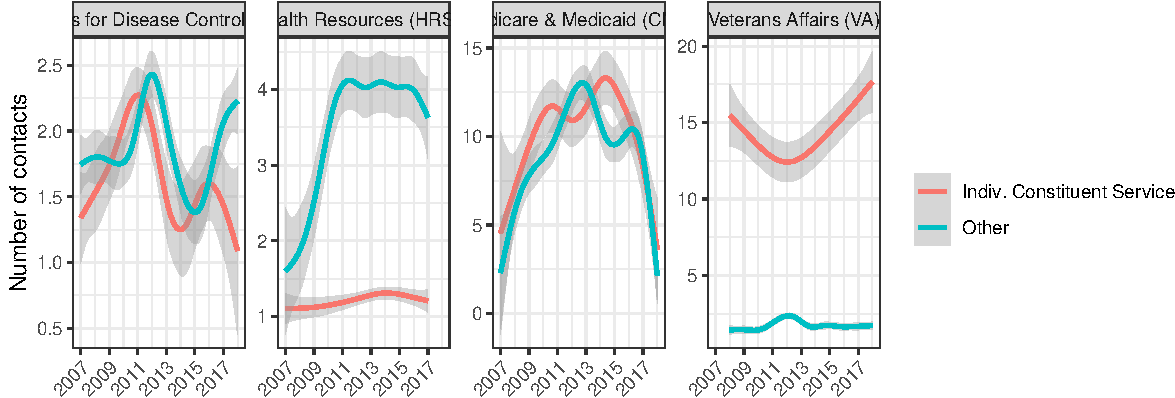
\includegraphics{Figs/n_per_year_agency-1} \end{center}

\begin{Shaded}
\begin{Highlighting}[]
\NormalTok{d1 }\OperatorTok{\%\textgreater{}\%}
\StringTok{  }\KeywordTok{filter}\NormalTok{(party\_name }\OperatorTok{!=}\StringTok{ "Independent"}\NormalTok{) }\OperatorTok{\%\textgreater{}\%}\StringTok{ }
\StringTok{  }\KeywordTok{group\_by}\NormalTok{(icpsr, party\_name, agency, year) }\OperatorTok{\%\textgreater{}\%}\StringTok{ }
\StringTok{  }\KeywordTok{summarise}\NormalTok{(}\DataTypeTok{n\_per\_year\_agency =} \KeywordTok{sum}\NormalTok{(n\_per\_year\_agency\_type)) }\OperatorTok{\%\textgreater{}\%}
\StringTok{  }\KeywordTok{ggplot}\NormalTok{() }\OperatorTok{+}
\StringTok{  }\KeywordTok{aes}\NormalTok{(}\DataTypeTok{x =}\NormalTok{ year, }\DataTypeTok{color =}\NormalTok{ party\_name, }\DataTypeTok{y =}\NormalTok{ n\_per\_year\_agency) }\OperatorTok{+}
\StringTok{  }\CommentTok{\#geom\_line(aes(group= icpsr), alpha = .1) + }
\StringTok{  }\KeywordTok{geom\_smooth}\NormalTok{() }\OperatorTok{+}\StringTok{ }
\StringTok{  }\KeywordTok{labs}\NormalTok{(}\DataTypeTok{x =} \StringTok{""}\NormalTok{, }\DataTypeTok{y =} \StringTok{"Number of contacts"}\NormalTok{, }\DataTypeTok{color =} \StringTok{""}\NormalTok{) }\OperatorTok{+}\StringTok{ }
\StringTok{  }\KeywordTok{facet\_wrap}\NormalTok{(. }\OperatorTok{\textasciitilde{}}\StringTok{ }\NormalTok{agency, }\DataTypeTok{scales =} \StringTok{"free\_y"}\NormalTok{, }\DataTypeTok{nrow =} \DecValTok{1}\NormalTok{) }\OperatorTok{+}
\StringTok{  }\KeywordTok{scale\_x\_continuous}\NormalTok{(}\DataTypeTok{breaks =} \KeywordTok{seq}\NormalTok{(}\DecValTok{2007}\NormalTok{,}\DecValTok{2019}\NormalTok{, }\DecValTok{1}\NormalTok{)) }\OperatorTok{+}
\StringTok{  }\KeywordTok{scale\_color\_brewer}\NormalTok{(}\DataTypeTok{palette =} \StringTok{"RdBu"}\NormalTok{) }\OperatorTok{+}\StringTok{ }
\StringTok{  }\KeywordTok{theme}\NormalTok{(}\DataTypeTok{axis.text.x =} \KeywordTok{element\_text}\NormalTok{(}\DataTypeTok{angle =} \DecValTok{45}\NormalTok{, }\DataTypeTok{hjust =} \DecValTok{1}\NormalTok{))}
\end{Highlighting}
\end{Shaded}

\begin{center}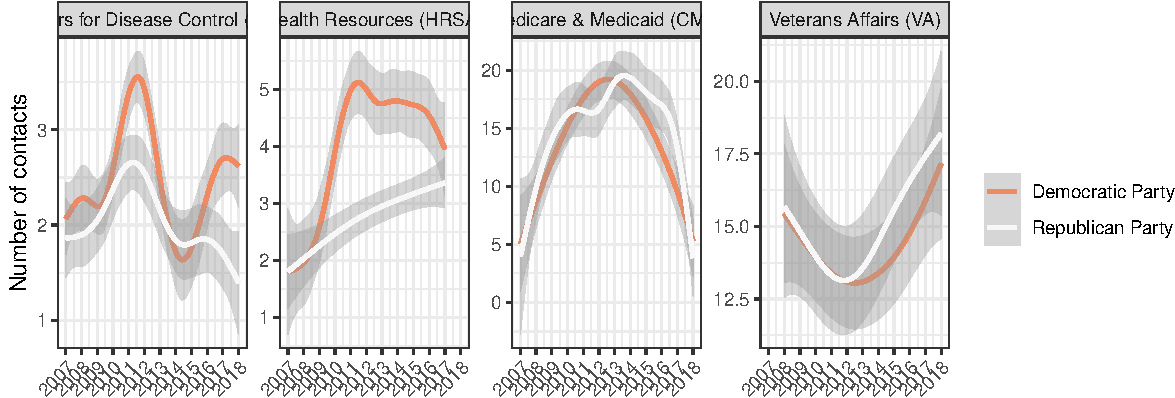
\includegraphics{Figs/n_per_year_agency-2} \end{center}

\hypertarget{percent-of-legislator-contacts-per-agency-per-year-2007-2017}{%
\subsection{Percent of legislator contacts per agency per year
2007-2017}\label{percent-of-legislator-contacts-per-agency-per-year-2007-2017}}

\begin{Shaded}
\begin{Highlighting}[]
\NormalTok{d1 }\OperatorTok{\%\textgreater{}\%}\StringTok{ }
\StringTok{  }\KeywordTok{ggplot}\NormalTok{() }\OperatorTok{+}
\StringTok{  }\KeywordTok{aes}\NormalTok{(}\DataTypeTok{x =}\NormalTok{ year, }\DataTypeTok{y =}\NormalTok{ percent\_type\_to\_agency, }\DataTypeTok{color =}\NormalTok{ constituent) }\OperatorTok{+}
\StringTok{  }\CommentTok{\#geom\_line(aes(group= icpsr), alpha = .1) + }
\StringTok{  }\KeywordTok{geom\_smooth}\NormalTok{() }\OperatorTok{+}\StringTok{ }
\StringTok{  }\KeywordTok{labs}\NormalTok{(}\DataTypeTok{x =} \StringTok{""}\NormalTok{, }\DataTypeTok{y =} \StringTok{"Percent of contacts"}\NormalTok{, }\DataTypeTok{color =} \StringTok{""}\NormalTok{) }\OperatorTok{+}\StringTok{ }
\StringTok{  }\KeywordTok{facet\_wrap}\NormalTok{(. }\OperatorTok{\textasciitilde{}}\StringTok{ }\NormalTok{agency, }\DataTypeTok{scales =} \StringTok{"free\_y"}\NormalTok{, }\DataTypeTok{nrow =} \DecValTok{1}\NormalTok{) }\OperatorTok{+}
\StringTok{  }\KeywordTok{scale\_x\_continuous}\NormalTok{(}\DataTypeTok{breaks =} \KeywordTok{seq}\NormalTok{(}\DecValTok{2007}\NormalTok{,}\DecValTok{2017}\NormalTok{, }\DecValTok{2}\NormalTok{)) }\OperatorTok{+}
\StringTok{  }\KeywordTok{theme}\NormalTok{(}\DataTypeTok{axis.text.x =} \KeywordTok{element\_text}\NormalTok{(}\DataTypeTok{angle =} \DecValTok{45}\NormalTok{, }\DataTypeTok{hjust =} \DecValTok{1}\NormalTok{))}
\end{Highlighting}
\end{Shaded}

\begin{center}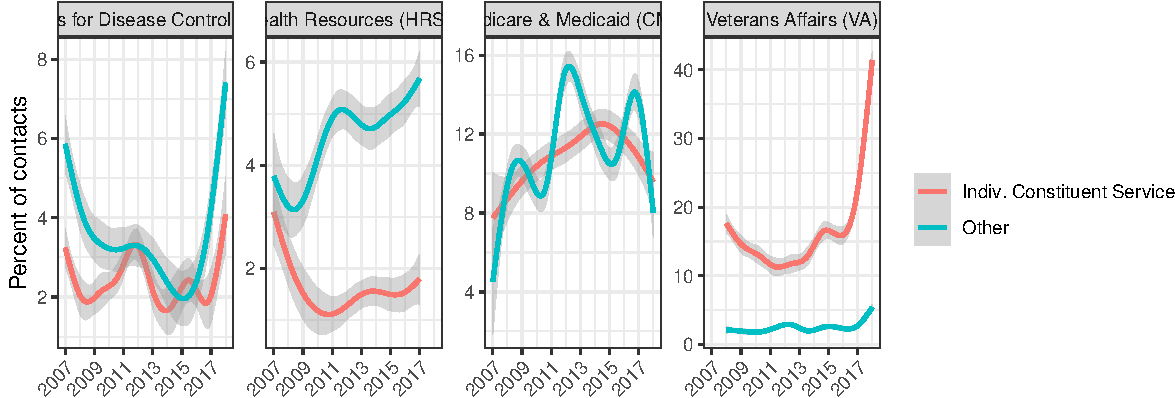
\includegraphics{Figs/percent_to_agency-1} \end{center}

\hypertarget{constituent-type-count}{%
\subsection{Constituent type count:}\label{constituent-type-count}}

\begin{Shaded}
\begin{Highlighting}[]
\KeywordTok{load}\NormalTok{(here}\OperatorTok{::}\KeywordTok{here}\NormalTok{(}\StringTok{"data"}\NormalTok{, }\StringTok{"dcounts\_min.Rdata"}\NormalTok{))}


\NormalTok{dcounts\_min}\OperatorTok{$}\NormalTok{agency }\OperatorTok{\%\textless{}\textgreater{}\%}\StringTok{ }
\StringTok{  }\KeywordTok{str\_replace}\NormalTok{(}\StringTok{"VA"}\NormalTok{, }\StringTok{"Veterans Affairs (VA)"}\NormalTok{) }\OperatorTok{\%\textgreater{}\%}\StringTok{ }
\StringTok{  }\KeywordTok{str\_replace}\NormalTok{(}\StringTok{"DHHS\_CMS"}\NormalTok{, }\StringTok{"Medicare \& Medicaid (CMS)"}\NormalTok{) }\OperatorTok{\%\textgreater{}\%}\StringTok{ }
\StringTok{  }\KeywordTok{str\_replace}\NormalTok{(}\StringTok{"DHHS\_CDC"}\NormalTok{, }\StringTok{"Centers for Disease Control (CDC)"}\NormalTok{) }\OperatorTok{\%\textgreater{}\%}\StringTok{ }
\StringTok{  }\KeywordTok{str\_replace}\NormalTok{(}\StringTok{"DHHS\_HRSA"}\NormalTok{, }\StringTok{"Health Resources (HRSA)"}\NormalTok{) }\OperatorTok{\%\textgreater{}\%}\StringTok{ }
\StringTok{  }\KeywordTok{str\_replace}\NormalTok{(}\StringTok{"Treasury\_IRS"}\NormalTok{, }\StringTok{"IRS"}\NormalTok{) }\OperatorTok{\%\textgreater{}\%}
\StringTok{  }\KeywordTok{str\_replace}\NormalTok{(}\StringTok{"NARA"}\NormalTok{, }\StringTok{"National Archives (NARA)"}\NormalTok{) }\OperatorTok{\%\textgreater{}\%}\StringTok{ }
\StringTok{  }\KeywordTok{str\_replace}\NormalTok{(}\StringTok{"DOL.*"}\NormalTok{, }\StringTok{"Labor (DOL VETS, SOL, OWCP, \& OFCCP)"}\NormalTok{) }\OperatorTok{\%\textgreater{}\%}\StringTok{ }
\StringTok{  }\KeywordTok{str\_replace}\NormalTok{(}\StringTok{"Treasury\_Fiscal"}\NormalTok{, }\StringTok{"Treasury Fiscal Service"}\NormalTok{) }\OperatorTok{\%\textgreater{}\%}\StringTok{ }
\StringTok{  }\KeywordTok{str\_replace}\NormalTok{(}\StringTok{"SSA"}\NormalTok{, }\StringTok{"Social Security (SSA)"}\NormalTok{)}

\KeywordTok{names}\NormalTok{(dcounts\_min) }\OperatorTok{\%\textless{}\textgreater{}\%}\StringTok{ }\KeywordTok{str\_replace}\NormalTok{(}\StringTok{"vet"}\NormalTok{, }\StringTok{"Veteran"}\NormalTok{) }\OperatorTok{\%\textgreater{}\%}
\StringTok{                            }\KeywordTok{str\_replace}\NormalTok{(}\StringTok{"hardship"}\NormalTok{, }\StringTok{"Hardship situation"}\NormalTok{) }\OperatorTok{\%\textgreater{}\%}\StringTok{ }
\StringTok{                            }\KeywordTok{str\_replace}\NormalTok{(}\StringTok{"lowincome"}\NormalTok{, }\StringTok{"Low income"}\NormalTok{)}\OperatorTok{\%\textgreater{}\%}
\StringTok{                            }\KeywordTok{str\_replace}\NormalTok{(}\StringTok{"military"}\NormalTok{, }\StringTok{"Military family or veteran"}\NormalTok{) }\OperatorTok{\%\textgreater{}\%}
\StringTok{                            }\KeywordTok{str\_replace}\NormalTok{(}\StringTok{"senior"}\NormalTok{, }\StringTok{"Senior"}\NormalTok{)}

\NormalTok{dcounts\_min }\OperatorTok{\%\textgreater{}\%}\StringTok{ }
\StringTok{  }\CommentTok{\# melt count vars to long}
\StringTok{  }\KeywordTok{select}\NormalTok{(agency, }\KeywordTok{starts\_with}\NormalTok{(}\StringTok{"per"}\NormalTok{)) }\OperatorTok{\%\textgreater{}\%}\StringTok{ }
\StringTok{  }\KeywordTok{gather}\NormalTok{(}\StringTok{"type"}\NormalTok{, }\StringTok{"count"}\NormalTok{, }\OperatorTok{{-}}\NormalTok{agency) }\OperatorTok{\%\textgreater{}\%}
\StringTok{  }\KeywordTok{mutate}\NormalTok{(}\DataTypeTok{type =}\NormalTok{ type }\OperatorTok{\%\textgreater{}\%}\StringTok{ }\KeywordTok{str\_remove}\NormalTok{(}\StringTok{".*\_"}\NormalTok{)) }\OperatorTok{\%\textgreater{}\%}
\StringTok{  }\CommentTok{\# count}
\StringTok{  }\KeywordTok{group\_by}\NormalTok{(agency, type) }\OperatorTok{\%\textgreater{}\%}\StringTok{ }
\StringTok{  }\KeywordTok{summarize}\NormalTok{(}\DataTypeTok{count =} \KeywordTok{sum}\NormalTok{(count)) }\OperatorTok{\%\textgreater{}\%}\StringTok{ }
\StringTok{  }\KeywordTok{ungroup}\NormalTok{() }\OperatorTok{\%\textgreater{}\%}
\StringTok{  }\KeywordTok{filter}\NormalTok{(count }\OperatorTok{\textgreater{}}\StringTok{ }\DecValTok{0}\NormalTok{) }\OperatorTok{\%\textgreater{}\%}\StringTok{ }\CommentTok{\#select(type) \%\textgreater{}\% distinct()}
\StringTok{  }\KeywordTok{filter}\NormalTok{(type }\OperatorTok{\%in\%}\StringTok{ }\KeywordTok{c}\NormalTok{(}\StringTok{"Hardship situation"}\NormalTok{,}
  \CommentTok{\#"Military family or veteran",}
  \StringTok{"Senior"}\NormalTok{,}
  \StringTok{"Veteran"}\NormalTok{,}
  \StringTok{"Low income"}\NormalTok{)) }\OperatorTok{\%\textgreater{}\%}
\StringTok{  }\KeywordTok{group\_by}\NormalTok{(type) }\OperatorTok{\%\textgreater{}\%}\StringTok{ }
\StringTok{  }\KeywordTok{add\_count}\NormalTok{(}\DataTypeTok{name =} \StringTok{"n\_agency"}\NormalTok{) }\OperatorTok{\%\textgreater{}\%}\StringTok{ }\CommentTok{\# n agencies per type }
\StringTok{    }\KeywordTok{ungroup}\NormalTok{() }\OperatorTok{\%\textgreater{}\%}
\StringTok{  }\KeywordTok{ggplot}\NormalTok{() }\OperatorTok{+}\StringTok{ }
\StringTok{  }\KeywordTok{aes}\NormalTok{(}\DataTypeTok{y =}\NormalTok{ count, }\DataTypeTok{x =}\NormalTok{ agency, }\DataTypeTok{label =}\NormalTok{ count, }\DataTypeTok{width =} \FloatTok{.15}\OperatorTok{*}\NormalTok{n\_agency) }\OperatorTok{+}
\StringTok{  }\KeywordTok{geom\_col}\NormalTok{(}\DataTypeTok{position =} \StringTok{"dodge"}\NormalTok{, }\DataTypeTok{preserve =} \StringTok{"single"}\NormalTok{) }\OperatorTok{+}
\StringTok{  }\KeywordTok{geom\_text}\NormalTok{(}\DataTypeTok{hjust =} \FloatTok{{-}.1}\NormalTok{) }\OperatorTok{+}\StringTok{ }
\StringTok{  }\KeywordTok{coord\_flip}\NormalTok{()}\OperatorTok{+}\StringTok{ }
\StringTok{  }\KeywordTok{scale\_y\_continuous}\NormalTok{(}\DataTypeTok{expand =} \KeywordTok{expand\_scale}\NormalTok{(}\DataTypeTok{mult =}  \KeywordTok{c}\NormalTok{(}\DecValTok{0}\NormalTok{,.}\DecValTok{2}\NormalTok{))) }\OperatorTok{+}\StringTok{ }\CommentTok{\# pad y axis so there is room for n text}
\StringTok{    }\KeywordTok{labs}\NormalTok{(}\DataTypeTok{y =} \StringTok{"Number of Constituent Service Letters"}\NormalTok{, }\CommentTok{\#paste("Letters on Behalf", type), }
         \DataTypeTok{x =} \StringTok{"Agency"}\NormalTok{) }\OperatorTok{+}\StringTok{ }
\StringTok{  }\KeywordTok{facet\_wrap}\NormalTok{(}\StringTok{"type"}\NormalTok{, }\DataTypeTok{scales =} \StringTok{"free"}\NormalTok{, }\DataTypeTok{ncol =} \DecValTok{1}\NormalTok{) }\OperatorTok{+}
\StringTok{  }\KeywordTok{theme\_bw}\NormalTok{() }\OperatorTok{+}\StringTok{ }
\StringTok{  }\KeywordTok{theme}\NormalTok{(}\DataTypeTok{panel.grid.minor.y =} \KeywordTok{element\_blank}\NormalTok{(),}
        \DataTypeTok{panel.grid.major.y =} \KeywordTok{element\_blank}\NormalTok{())}
\end{Highlighting}
\end{Shaded}

\begin{figure}

{\centering 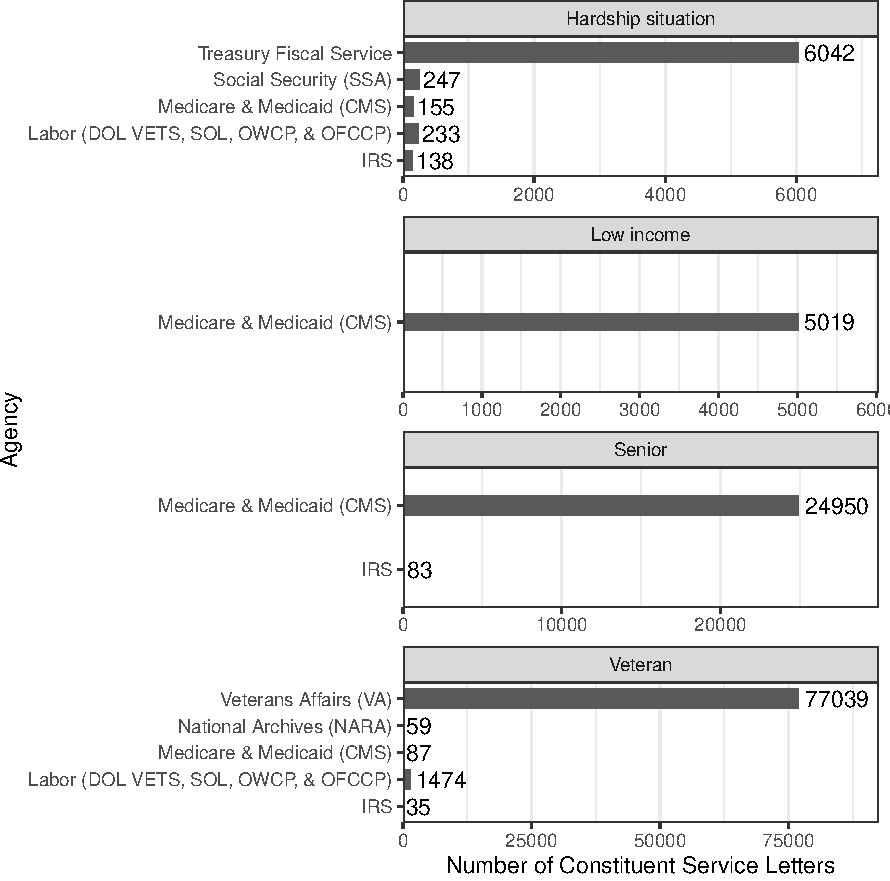
\includegraphics{Figs/constituent_type_count-1} 

}

\caption{Number of Legislator Letters per Type of Constituent}\label{fig:constituent_type_count}
\end{figure}

\hypertarget{constituent-type-share-of-total-per-agency}{%
\section{Constituent type share of total per
agency}\label{constituent-type-share-of-total-per-agency}}

\begin{Shaded}
\begin{Highlighting}[]
\NormalTok{dcounts\_min }\OperatorTok{\%\textgreater{}\%}\StringTok{ }
\StringTok{  }\CommentTok{\#select({-}per\_icpsr\_chamber\_year\_agency\_type) \%\textgreater{}\%}
\StringTok{  }\KeywordTok{group\_by}\NormalTok{(agency) }\OperatorTok{\%\textgreater{}\%}\StringTok{ }
\StringTok{  }\KeywordTok{summarise}\NormalTok{(}\KeywordTok{across}\NormalTok{(}\KeywordTok{starts\_with}\NormalTok{(}\StringTok{"per\_"}\NormalTok{), sum)) }\OperatorTok{\%\textgreater{}\%}\StringTok{ }
\StringTok{  }\KeywordTok{gather}\NormalTok{(}\DataTypeTok{key =}\NormalTok{ type, }\DataTypeTok{value =}\NormalTok{ count, }\OperatorTok{{-}}\NormalTok{agency) }\OperatorTok{\%\textgreater{}\%}
\StringTok{  }\KeywordTok{mutate}\NormalTok{(}\DataTypeTok{type =} \KeywordTok{str\_remove\_all}\NormalTok{(type, }\StringTok{".*\_"}\NormalTok{) }\OperatorTok{\%\textgreater{}\%}\StringTok{ }\KeywordTok{str\_replace}\NormalTok{(}\StringTok{"type"}\NormalTok{, }\StringTok{"All"}\NormalTok{) ) }\OperatorTok{\%\textgreater{}\%}
\StringTok{  }\KeywordTok{group\_by}\NormalTok{(agency) }\OperatorTok{\%\textgreater{}\%}\StringTok{ }
\StringTok{  }\KeywordTok{mutate}\NormalTok{(}\DataTypeTok{agencycount =} \KeywordTok{sum}\NormalTok{(count)) }\OperatorTok{\%\textgreater{}\%}
\StringTok{  }\KeywordTok{filter}\NormalTok{(count }\OperatorTok{\textgreater{}}\DecValTok{0}\NormalTok{, agencycount }\OperatorTok{\textgreater{}}\StringTok{ }\NormalTok{count) }\OperatorTok{\%\textgreater{}\%}
\StringTok{  }\KeywordTok{group\_by}\NormalTok{(agency) }\OperatorTok{\%\textgreater{}\%}\StringTok{ }
\StringTok{  }\KeywordTok{add\_count}\NormalTok{(}\DataTypeTok{name =} \StringTok{"n\_types"}\NormalTok{) }\OperatorTok{\%\textgreater{}\%}\StringTok{ }
\StringTok{  }\KeywordTok{ggplot}\NormalTok{() }\OperatorTok{+}\StringTok{ }
\StringTok{  }\KeywordTok{aes}\NormalTok{(}\DataTypeTok{x =}\NormalTok{ agency, }\DataTypeTok{y =}\NormalTok{ count, }\DataTypeTok{fill =} \KeywordTok{factor}\NormalTok{(type), }\DataTypeTok{label =}\NormalTok{ count, }\DataTypeTok{width =} \FloatTok{.2}\OperatorTok{*}\NormalTok{n\_types) }\OperatorTok{+}
\StringTok{  }\KeywordTok{geom\_col}\NormalTok{(}\DataTypeTok{position =} \StringTok{"dodge"}\NormalTok{) }\OperatorTok{+}
\StringTok{  }\CommentTok{\#geom\_text(position = "dodge", hjust = 0) + }
\StringTok{  }\KeywordTok{coord\_flip}\NormalTok{()}\OperatorTok{+}\StringTok{ }
\StringTok{  }\KeywordTok{scale\_y\_continuous}\NormalTok{()}\OperatorTok{+}\CommentTok{\#expand = expand\_scale(mult =  c(0,.2))) +}
\StringTok{    }\KeywordTok{labs}\NormalTok{(}\DataTypeTok{y =} \StringTok{""}\NormalTok{, }
         \DataTypeTok{x =} \StringTok{"Agency"}\NormalTok{,}
         \DataTypeTok{fill =} \StringTok{"Type of Constituent"}\NormalTok{) }\OperatorTok{+}\StringTok{ }
\StringTok{  }\KeywordTok{facet\_wrap}\NormalTok{(}\StringTok{"agency"}\NormalTok{, }\DataTypeTok{scales =} \StringTok{"free"}\NormalTok{, }\DataTypeTok{ncol =} \DecValTok{1}\NormalTok{) }\OperatorTok{+}
\StringTok{  }\KeywordTok{theme\_bw}\NormalTok{() }\OperatorTok{+}\StringTok{ }
\StringTok{  }\KeywordTok{theme}\NormalTok{(}\DataTypeTok{panel.border =} \KeywordTok{element\_blank}\NormalTok{(),}
        \DataTypeTok{axis.ticks =} \KeywordTok{element\_blank}\NormalTok{(),}
         \DataTypeTok{panel.grid.minor.y =} \KeywordTok{element\_blank}\NormalTok{(),}
        \DataTypeTok{panel.grid.major.y =} \KeywordTok{element\_blank}\NormalTok{(),}
        \DataTypeTok{strip.background =} \KeywordTok{element\_blank}\NormalTok{(),}
        \DataTypeTok{strip.text.x =} \KeywordTok{element\_blank}\NormalTok{())}
\end{Highlighting}
\end{Shaded}

\begin{figure}

{\centering 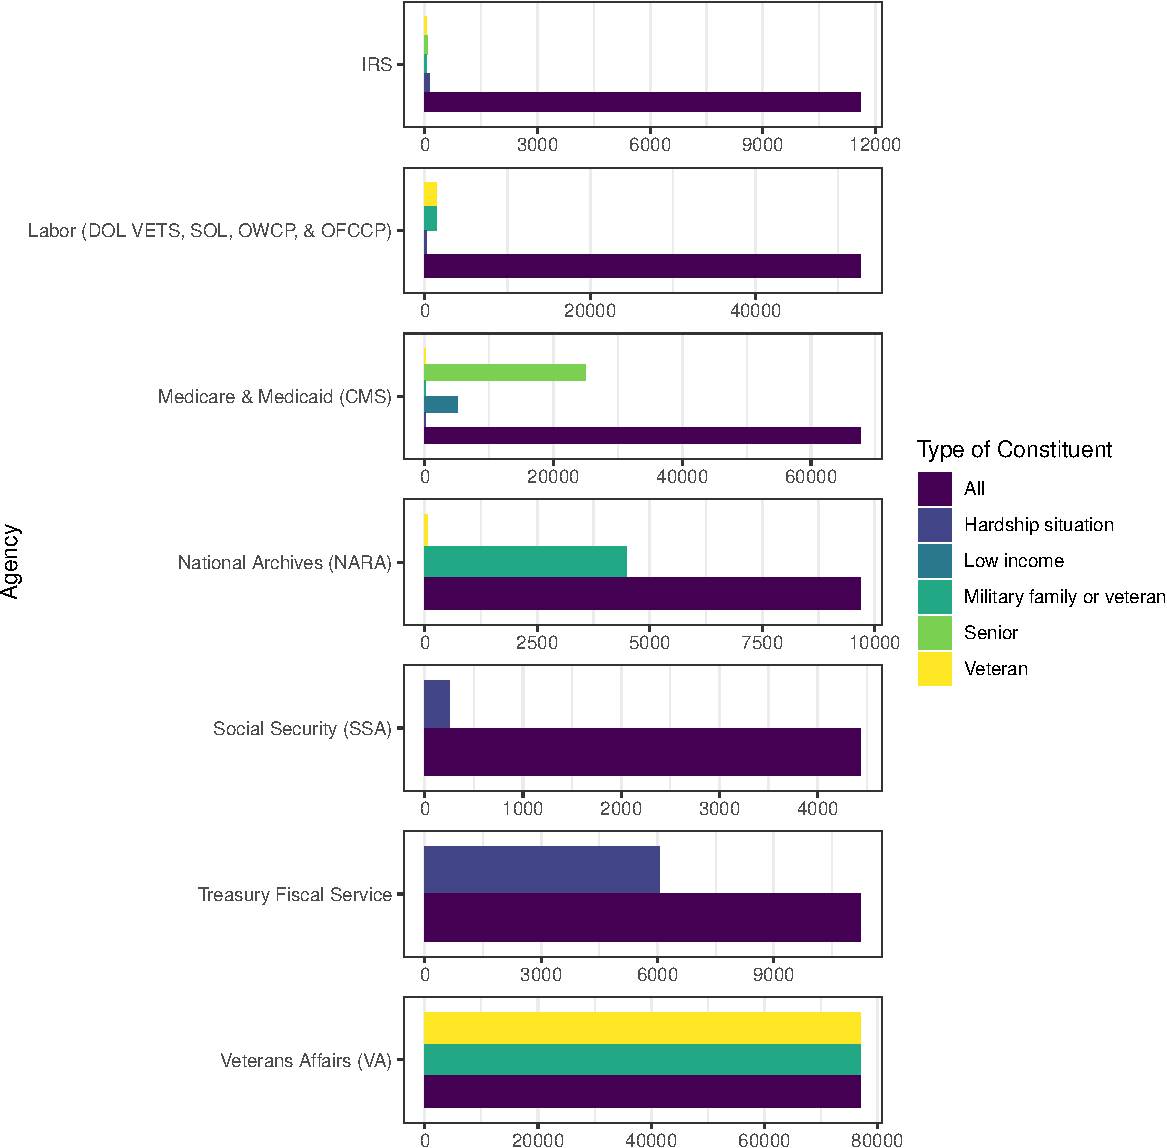
\includegraphics[width=1\linewidth]{Figs/constituent_type_share-1} 

}

\caption{Share of Legislator Contacts by Type of Constituent}\label{fig:constituent_type_share}
\end{figure}

\hypertarget{member-congress-percentiles}{%
\section{Member-Congress
Percentiles}\label{member-congress-percentiles}}

\begin{Shaded}
\begin{Highlighting}[]
\KeywordTok{load}\NormalTok{(here}\OperatorTok{::}\KeywordTok{here}\NormalTok{(}\StringTok{"data"}\NormalTok{, }\StringTok{"dcounts\_mid.Rdata"}\NormalTok{))}

\NormalTok{dcounts }\OperatorTok{\%\textless{}\textgreater{}\%}\StringTok{ }\KeywordTok{filter}\NormalTok{(chamber }\OperatorTok{!=}\StringTok{ "President"}\NormalTok{)}

\NormalTok{dcounts }\OperatorTok{\%\textless{}\textgreater{}\%}\StringTok{ }\KeywordTok{select}\NormalTok{(chamber, last\_name, state\_abbrev, party\_name, congress, year, agency, icpsr, TYPE, }\KeywordTok{starts\_with}\NormalTok{(}\StringTok{"per\_"}\NormalTok{)) }


\CommentTok{\# save(dcounts, file = here::here("data" , "dcounts\_mid.Rdata"))}


\NormalTok{dcounts }\OperatorTok{\%\textless{}\textgreater{}\%}\StringTok{ }
\StringTok{    }\KeywordTok{mutate}\NormalTok{(}\DataTypeTok{member\_state =} \KeywordTok{str\_c}\NormalTok{(last\_name, }\StringTok{", "}\NormalTok{, }\KeywordTok{str\_sub}\NormalTok{(party\_name, }\DecValTok{1}\NormalTok{, }\DecValTok{1}\NormalTok{), }\StringTok{"{-}"}\NormalTok{, state\_abbrev)) }

\NormalTok{percentplot \textless{}{-}}\StringTok{ }\ControlFlowTok{function}\NormalTok{(var, title, x)\{}
  
\NormalTok{  dcounts}\OperatorTok{$}\NormalTok{var \textless{}{-}}\StringTok{ }\NormalTok{var}

\NormalTok{  dcounts }\OperatorTok{\%\textgreater{}\%}
\StringTok{      }\KeywordTok{group\_by}\NormalTok{(member\_state, chamber, congress) }\OperatorTok{\%\textgreater{}\%}\StringTok{ }\KeywordTok{summarise}\NormalTok{(}\DataTypeTok{n =} \KeywordTok{sum}\NormalTok{(var)) }\OperatorTok{\%\textgreater{}\%}
\StringTok{      }\KeywordTok{group\_by}\NormalTok{(member\_state, chamber) }\OperatorTok{\%\textgreater{}\%}\StringTok{ }\KeywordTok{mutate}\NormalTok{(}\DataTypeTok{mean =} \KeywordTok{mean}\NormalTok{(n)) }\OperatorTok{\%\textgreater{}\%}\StringTok{ }\KeywordTok{ungroup}\NormalTok{() }\OperatorTok{\%\textgreater{}\%}\StringTok{ }
\StringTok{      }\KeywordTok{group\_by}\NormalTok{(chamber) }\OperatorTok{\%\textgreater{}\%}\StringTok{ }\KeywordTok{mutate}\NormalTok{(}\DataTypeTok{Percentile =} \KeywordTok{ntile}\NormalTok{(mean, }\DecValTok{100}\NormalTok{)) }\OperatorTok{\%\textgreater{}\%}\StringTok{ }
\StringTok{    }\KeywordTok{arrange}\NormalTok{(}\OperatorTok{{-}}\NormalTok{Percentile) }\OperatorTok{\%\textgreater{}\%}\StringTok{ }
\StringTok{    }\NormalTok{dplyr}\OperatorTok{::}\KeywordTok{select}\NormalTok{(member\_state, Percentile, mean, chamber) }\OperatorTok{\%\textgreater{}\%}\StringTok{ }\KeywordTok{distinct}\NormalTok{() }\OperatorTok{\%\textgreater{}\%}\StringTok{ }
\StringTok{      }\KeywordTok{ggplot}\NormalTok{() }\OperatorTok{+}\StringTok{ }
\StringTok{      }\KeywordTok{geom\_col}\NormalTok{(}\KeywordTok{aes}\NormalTok{(}\DataTypeTok{x =}\NormalTok{ Percentile, }\DataTypeTok{y =}\NormalTok{ mean), }\DataTypeTok{color =} \StringTok{"grey"}\NormalTok{, }\DataTypeTok{position =} \StringTok{"dodge"}\NormalTok{) }\OperatorTok{+}\StringTok{ }
\StringTok{    }\KeywordTok{geom\_point}\NormalTok{(}\KeywordTok{aes}\NormalTok{(}\DataTypeTok{x =}\NormalTok{ Percentile, }\DataTypeTok{y =}\NormalTok{ mean), }\DataTypeTok{color =} \StringTok{"grey"}\NormalTok{) }\OperatorTok{+}\StringTok{ }
\StringTok{    }\KeywordTok{geom\_text}\NormalTok{(}\KeywordTok{aes}\NormalTok{(}\DataTypeTok{x =}\NormalTok{ Percentile, }\DataTypeTok{y =}\NormalTok{ mean, }\DataTypeTok{label =} \KeywordTok{ifelse}\NormalTok{(Percentile }\OperatorTok{\textgreater{}}\StringTok{ }\DecValTok{90}\NormalTok{, member\_state, }\StringTok{""}\NormalTok{)), }\DataTypeTok{check\_overlap =}\NormalTok{ T, }\DataTypeTok{size =} \DecValTok{2}\NormalTok{, }\DataTypeTok{hjust =} \StringTok{"inward"}\NormalTok{) }\OperatorTok{+}\StringTok{ }
\StringTok{      }\KeywordTok{facet\_grid}\NormalTok{(. }\OperatorTok{\textasciitilde{}}\StringTok{ }\NormalTok{chamber , }\DataTypeTok{scales =} \StringTok{"free\_y"}\NormalTok{) }\OperatorTok{+}\StringTok{ }\KeywordTok{theme\_bw}\NormalTok{() }\OperatorTok{+}
\StringTok{    }\KeywordTok{labs}\NormalTok{(}\CommentTok{\#title = "Average Legislator Requests per Congress by Percentile",}
      \DataTypeTok{title =}\NormalTok{ title,}
         \DataTypeTok{y =} \StringTok{""}\NormalTok{,}
         \DataTypeTok{x =}\NormalTok{ x)}
\NormalTok{\}}


\KeywordTok{percentplot}\NormalTok{(dcounts}\OperatorTok{$}\NormalTok{per\_icpsr\_chamber\_year\_agency\_vet, }\StringTok{"Veterans"}\NormalTok{, }\DataTypeTok{x =} \StringTok{"Percentile"}\NormalTok{)}
\CommentTok{\#percentplot(dcounts$per\_icpsr\_chamber\_year\_agency\_military, "Military Families, Personal, and Veterans")}
\KeywordTok{percentplot}\NormalTok{(dcounts}\OperatorTok{$}\NormalTok{per\_icpsr\_chamber\_year\_agency\_senior, }\StringTok{"Seniors"}\NormalTok{, }\DataTypeTok{x =} \StringTok{"Percentile"}\NormalTok{)}
\KeywordTok{percentplot}\NormalTok{(dcounts}\OperatorTok{$}\NormalTok{per\_icpsr\_chamber\_year\_agency\_hardship, }\StringTok{"Constituents Experiencing Hardship"}\NormalTok{, }\DataTypeTok{x =} \StringTok{"Percentile"}\NormalTok{)}
\KeywordTok{percentplot}\NormalTok{(dcounts}\OperatorTok{$}\NormalTok{per\_icpsr\_chamber\_year\_agency\_lowincome, }\StringTok{"Low Income Constituents"}\NormalTok{, }\DataTypeTok{x =} \StringTok{"Percentile"}\NormalTok{)}
\end{Highlighting}
\end{Shaded}

\begin{figure}

{\centering 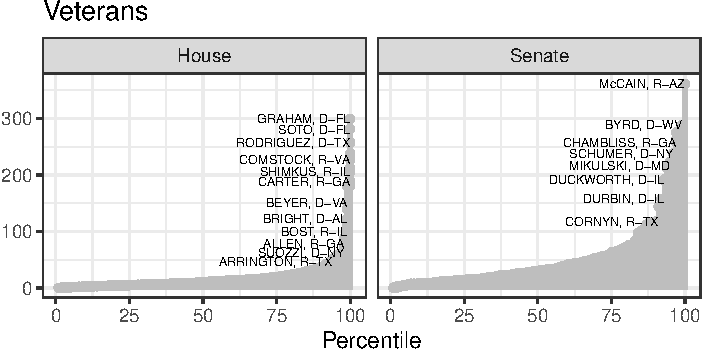
\includegraphics{Figs/percent_correp-1} 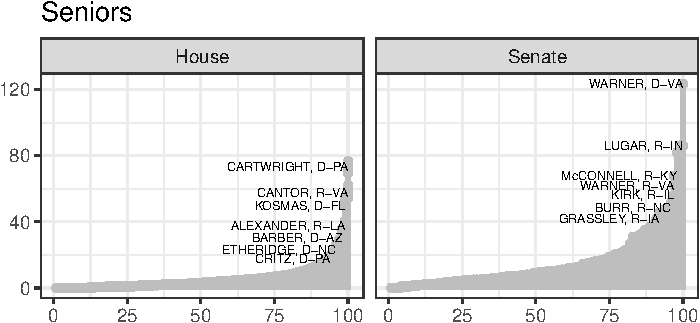
\includegraphics{Figs/percent_correp-2} 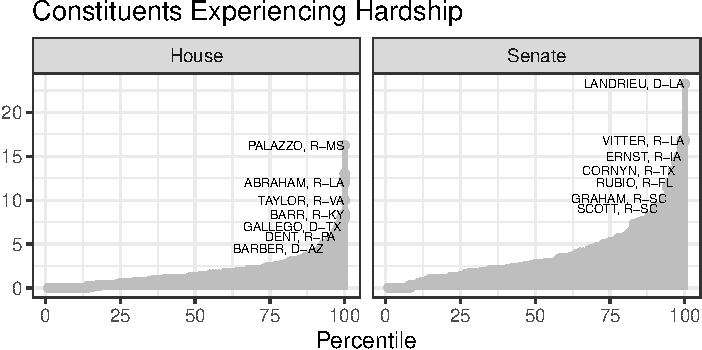
\includegraphics{Figs/percent_correp-3} 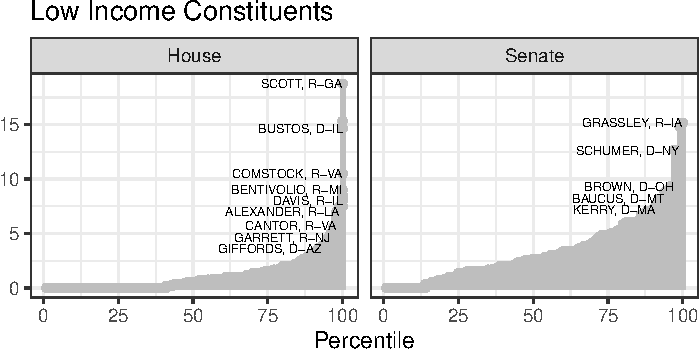
\includegraphics{Figs/percent_correp-4} 

}

\caption{Average Legislator Requests per Congress by Constituent Type}\label{fig:percent_correp}
\end{figure}

\hypertarget{todo}{%
\section{TODO}\label{todo}}

\begin{quote}
Maybe also any interesting patterns in the volume of total letters on
behalf of constituent types over time? Bars for each Congress broken
down by constituent type Basically, this would show how many letters
there are on behalf of different constituent types, where the letters
are in the agencies, who is writing the letters, and when the letters
were written.
\end{quote}

\end{document}
